\chapter{Озеро Гнилуша и окрестности}

%Я веду повествование потихоньку, почти не касаясь пока ни раскопок, ни Городков и того, что прочат в их следы – городищ. Если начать всё это трогать сразу, выйдет путаница. Но последовательное изложение разных положений не даст путанице просочиться в рассуждения.

%Нет смысла пускаться в изучение источников, вычислять летописные Городки и прочие древности, не познакомившись с местностью, причем постепенно, проверяя каждый свой шаг. Верно ли ступили? Верно ли название на карте?

%Гнилуша доставила мне много хлопот и заставила переписать еще более страниц. Поначалу я считал Гнилушей водоем, отмеченный так на картах. Потом я увлекся наложением карт, и по карте Шуберта выходило, что русла «современной» Гнилуши нет, зато есть водоем севернее – сейчас там, под пригорком с улицей Деснянской, на лугу лежат участки огородов и находится выгон. Пасутся лошади, коровы. 

%Водоем этот выглядел как буква «Г», верхней палочкой повернутая налево, а южнее был почти точно такой же водоем, но меньший. Гошкевич же, оставивший в докладе своем память о краеведческой вылазке сюда, в конце 19 века, писал:

%\begin{quotation}
%Все идя по-над долиною, мы подошли к высоким валам городища князя Симеона Олельковича: тылом городище обращено к бору, находясь от него в расстоянии нескольких десятков саженей, а с противоположной стороны оно примыкает к речке Гнилуше, то есть тому озерцу, которое на карте имеет форму прямого угла.
%\end{quotation}

%Я бульдожьей хваткой вцепился в этот прямой угол и, доверяя карте Шуберта, придумал себе, что на том поле, где теперь выгон, и даже залезая на Выгуровщину почти до улицы Довженко, существовала истинная Гнилуша, а современная это – другой водоем, быть может рукотворно возникший в начале 20 века. 

%Придумал – сказано грубо. Я пользовался логическими рассуждениями, на основании доступных мне источников. 

%К тому же в том поле на некоторых современных картах было отмечено урочище Городище, так же называется и одна из тамошних улиц. В поле проложены дороги,  связывающие земельные участки – некоторые уже застраиваются, однако на 2016 год местность еще сохраняет луговой свой вид.

%Несколько недель я потратил, чтобы нарисовать разные векторные карты и написать две главы, одну про истинную Гнилушу, другую про Гнилушу Мнимую, как я окрестил Гнилушу, обозначенную на картах. Работа над картами затянулась, потому что лето 2016 года выдалось очень жарким, и я должен был переждать жару, дабы отправиться на велике для полевых исследований.

%Думал, что сделал открытие. Все-то полагают – «городище» на берегу одного водоема, а оно было на берегу другого!

%Впрочем мне поныне неясно, сколь описанные в разные времена «городища» совпадают по местоположению.

%Когда я приступил к окончательной, как мне казалось, правке глав про Гнилуши, я уже снова сомневался. К тому времени уверенность в правильности карты Шуберта сильно во мне поколебалась. Я заметил, что она сильно искажает расстояния около лежащего к северо-востоку от села Троещины села Погребов. 

%Закрались сомнения относительно точности отражения на карте и Троещины с Выгуровщиной. Прудок протекал не так. Между тем берег болота – будущего Алмазного озера – был показан верно, равно как озеро Радунка. Одни объекты при наложении на современную карту оказывались на тех же местах, другие – много дальше, причем таким образом, что это означало ошибочность самой карты.

%Вернуться к общепринятой трактовке Гнилуши меня заставила та же карта Шуберта. Я разглядел на ней пометку «Кл» (кладбище) на северной околице Выгуровщины. К северо-западу от кладбища и был нарисован водоем в виде «Г» с повернутой палочкой.

%Такое же положение занимает «современная» Гнилуша относительно Выгуровского кладбища! 

%А я знал, что тогда, в середине 19 века, Выгуровщина была застроена только по широту нижнего, южного конца Гнилуши. Сопоставив карту Шуберта и современную умозрительно, без наложения одной на другую, я понял, что «Г»-образный водоем это и есть современная Гнилуша, разве только последняя лишилась своей верхней палочки.

%Пересматривать свои представления каждый раз мне не трудно, а грустно. И пришлось снова переписывать главы, связанные с Гнилушей – устранять придуманную мною в поле «истинную Гнилушу», возвращать прежнее значение Гнилуши, которую считал «мнимой». Однако простой откат к прошлым представлениям стал невозможен – я обогатился новыми знаниями и согласно им должен был многое изменить.
 
%Хорошо хоть этот пересмотр мнения в обратную сторону произошел у меня до выпуска очередной редакции книги, а то бы пустил выдумку по миру гулять!

Поглядим на кусок плана 1914 года:

\begin{center}
\includegraphics[width=\linewidth]{chast-gorodki/gnilusha/gni1914.jpg}
\end{center}

Салатовым я обвел Гнилушу. Синим – «Западный Залив» (его западный же берег на карте Визикома 2006 года подписан как «урочище Моложи»). Если на карте Шуберта примерно там было основное русло Черторыи, то теперь, в 1914 году, это уже один из двух ее рукавов, причем уже почти оторванный от Черторыи мелью на севере.
 
Красный кружок – место, где было село Троещина на карте Шуберта. Как видим, после 1877 года Троещина сместилась на восток.

%Фиолетовым овалом я очень приблизительно и умозрительно очертил местность, где была Гнилуша истинная. Частично ее уже в 1914 заняли жилые дома, частично – поля-огороды, как и сейчас. Вероятно, в 1890 году, когда тут бродил Гошкевич, от Гнилуши еще оставалось что-то, по крайней мере в поле. Я говорю это не без причины, об этом впрочем позже.

А с 1914 по 2016-й, Гнилуша в южной части сократилась метров на 180, прежде она доходила до широты чуть южнее\footnote{50°30'18"N 30°34'39"E} кладбища, до угла улицы Димитрова (где дома 9, 7, 5), а теперь оканчивается выше его.

По виду это отрезок полевой реки. Южный конец его засыпан, северный упирается в грунтовую дорогу, что идет от Выгуровщины на запад к Черторые, через поле, перерубая «Западный Залив». Дорога эта называется улицей Коцюбинского. «Западный Залив» ни сейчас, ни по карте 1914 года не поворачивает на восток ко Гнилуше, поэтому Гнилушу нельзя считать его продолжением, хотя оба водоема очень похожи – длинные старицы, заросшие зеленой тиной. 

Да что говорить, давайте туда отправимся и посмотрим. Чтобы местность не возникла в воображении просто так, оторванным островом, затронем и смежную, тем паче она нам тоже потом пригодится. Я буду катить на велике, а вы садитесь на багажник. Ничего, что трясет – зато с ветерком.

Мне удобней ехать к Выгуровщине от перекрестка проспекта Ватутина и улицы Бальзака. Я пересекаю линию скоростного трамвая – вижу их нечасто, наверное потому, что не успеваю заметить, такая у них скорость большая. Бетонным забором огороженные рельсы, по ним ходит обычный трамвай – вот вам и скоростной. Такой же на Борщаге.

Справа шумит трасса, слева лежит пересеченное грунтовками поле с рощицами, на современных картах подписанное как «урочище Вязки», за ним темнеет огромный залив Десенки. В той же стороне остался Московский мост. Пока далеко не отъехали, остановлюсь у обочины, достану из рюкзака термос с прохладной водой, попью и расскажу, что здесь было раньше и заодно про речку с бурой водой.

До постройки в 1976 году Московского моста, чуть южнее его присоединения к западному берегу острова Муромца, было место загородного отдыха и пристань «Выгуровщина». Туда с деревянного Спасского причала на Подоле (около Ильинской церкви) каждые полчаса по Днепру ходил катер. Если говорить в высшей степени научно, то теплоход марки «Москвич» – где нижняя палуба крытая, никакие брызги не страшны, а верхняя – просто с навесом. 

А со стороны села Выгуровщины, через Десенку была переправа на Муромец, по которой к пристани крестьяне приносили на продажу всяческую снедь. Стоял там и продуктовый киоск. Севернее пристани, на Муромце, с сороковых годов работал дом отдыха «Дніпрові хвилі». После сооружения Московского моста, в 1978 году причал был еще на прежнем месте, в 79-м его перенесли на север от моста, к пляжу парка Дружбы Народов, а затем и вовсе упразднили. Старая же переправа от села Выгуровщины через узкую тогда Черторыю была немного северней черторыйского отрезка Московского моста. По полю шла к ней длинная грунтовка.

И севернее оной, у другой луки Десенки – а теперь, стало быть, между остатками Выгуровщины и проспектом Ватутина, пролегает русло с рыжей водой. Ей посвящена отдельная глава.

%В середине 20 века эта речка была заметна еще в чистом поле там, где теперь дома по улица Бальзака 4, 9. Но долгого озера, что между номером 9 и Ватутина, рядом с развязками и остановками – раньше не было. С бывшей речкой пересекается лишь его западный берег. Нынешняя глубина чуть выше щиколоток, ширина русла несколько метров, оно обросло по берегам деревьями, а вверх по течению теряется в поле, куда я не смог последовать на велосипеде, когда исследовал местность. Русло бурой речки есть на карте лоций Днепра в районе Киева 1914, однако мне неясно, где ее исток.

Вот я попил водички из термоса и готов крутить педали дальше. По нечетной стороне улицы Бальзака добираемся к разным автомастерским и магазинам. Автобусная остановка с романтичным названием «Автостоянка». Сворачиваем на узкую улицу Карла Маркса – начинается Выгуровщина, уцелевший западный её кусочек. Слева – добротный частный сектор, крепкие дома с побеленными стенами. У многих во дворах похожие на склепы входы в погреба. Такое не увидишь в городском частном секторе, например на Ширме или Зверинце. А тут село, другое дело.

Справа тянется ограда Выгуровского кладбища. Кресты белые, голубые. Словно люди стоят в рубашках, расставив руки. Надгробия из полированного черного мрамора редки. Выкрашенный в золотой цвет памятник – солдат стоит преклонив колено, с непокрытой головой, в руке держит знамя. Это мемориал воинам Великой Отечественной войны, погибшим при освобождении сел Выгуровщины и Троещины. Через зелень чахлых березок проглядывает Троицкий собор, в то место Соболев перенес старую церковь.

У ограды притулилась низенькая автобусная остановка, сохранившая имя села – «с. Выгуровщина». Эдакий поставленный открытой частью к улице короб с длинной дощатой лавкой внутри. Лавка почти вровень с асфальтом, и когда садишься, поднимаются колени. Козырек издевательски короток, тени не дает, от дождя не бережет. С другой стороны – тоже остановка, только навес повыше, и козырек поумнее.

И это уже перекресток улиц Довженко и Карла Маркса. Мы поворачиваем налево по Довженко. Сей отрезок улицы – грунтовка в ширину автомобиля, между деревянных заборов. Очень скоро мы оказываемся на западном краю села, небольшом пригорке. Тут и было «городище», раскопанное в конце 19 века Завитневичем, о чем расскажу позже.

Эта возвышенность на восточном берегу Гнилуши давно застроена, но входит в зону охраны археологического культурного слоя 1-й категории памятника археологии «Городок Песочный». Непонятно, что тут осталось охранять. А вообще вся местность между селами Выгуровщиной с Троещиной по левый берег Десенки считается зоной охраны археологического культурного слоя второй категории – мол, для сохранения возможных тут древностей и дальнейшего изучения оных.

Но вот мы на пригорке. Направо тянутся заборы Выгуровщины, прямо – зеленеет, за камышами, озеро Гнилуша. За ним и левее простирается поле. Далеко видны деревья, за ними можно разглядеть опоры Московского моста, да по ту сторону Днепра – вышку телецентра. Деревья Муромца, Труханова закрывают вид на зеленые холмы Кирилловских высот. Хорошо просматриваются однако верха холмов лежащих напротив Приорки с Курёневкой. 

Вдоль озера на возвышенном, метра три, восточном берегу, стоят заборы частных усадеб. Между ними и водой идет грунтовка, затем тропка. Там местные жители пасут коз и сжигают листья. Озеро длинное, вытянутое с севера на юг, почти всё покрыто зеленой ряской.

Шелестит густой камыш, вода в плесах очень спокойная, дно не просматривается, и кажется, что на своем протяжении Гнилуша достаточно глубока, поскольку в единообразии русла не заметны отмели.

Западный берег низкий, переходит в степь. На карте Визикома 2006 года этот берег подписан как «урочище Сытняки». До Черторыи отсюда около шестисот метров на запад. Возле озера – домик и выгон для лошадей. Чуть южнее выгона, близ самого берега, ученые поставили памятный знак, камень с цитатой из летописи, на старославянском, где сказано, что Ярослав договорился о мире с Мстиславом, у Городца, и разделили они земли по Днепру. Не беда, что летопись молчит о месте Городца.

Кстати никто словом не обмолвится, что в ста метрах южнее памятного знака таки приметно городище\footnote{\textasciitilde{}50°30'28.2"N 30°34'33.85"E}! О нем я нигде не читал и не слышал, однако оно весьма очевидно. Вдоль озера, впрочем не у самой воды, прослеживается ровный давний вал. Перпендикулярно ему – ров, берега коего заросли кустарником и мелкими деревцами. Трудно понять, что к чему.

На восточном берегу для осмотра доступна только узкая полоса между заборами и озером. 

Длина Гнилуши на 2017 год составляет 500 с копейками метров, ширина в среднем – 50. Южная часть водоема засыпана привезенным откуда-то торфом, затем дальнейшее русло, пересохшее и сглаженное, подходит к бетонному порталу коллектора, от коего некое русло идет на юго-запад. Оно совпадает в некоторых частях с современным руслом Рыжей речки, рассказ о которой я всё откладываю до отдельной главы.

\newpage
\begin{center}
\includegraphics[width=0.93\linewidth]{chast-gorodki/gnilusha/IMG_20160316_154028.jpg}

\textit{2016. Вид с южной части Гнилуши на южную околицу Выгуровщины, восточный берег озера. Справа и впереди находилось «городище», которое раскопал Завитневич.}
\end{center}

\begin{center}
\includegraphics[width=0.93\linewidth]{chast-gorodki/gnilusha/\myimgprefix IMG_20160316_154438.jpg}

\textit{2016. Дорога по восточному берегу Гнилуши.}
\end{center}

\newpage
\vspace*{\fill}
\begin{center}
\includegraphics[width=\linewidth]{chast-gorodki/gnilusha/s_IMG_20140806_134029.jpg}
\end{center}

\begin{center}
\includegraphics[width=\linewidth]{chast-gorodki/gnilusha/s_IMG_20140806_134052.jpg}

\textit{2014. Вид на западное городище со стороны озера.}
\end{center}
\vspace*{\fill}
\newpage
\vspace*{\fill}
\begin{center}
\includegraphics[width=\linewidth]{chast-gorodki/gnilusha/s_IMG_20140806_131518.jpg}
\end{center}

\begin{center}
\includegraphics[width=\linewidth]{chast-gorodki/gnilusha/s_IMG_20140806_131746.jpg}

\textit{Вид на Гнилушу с восточного берега, дорога по нему.}
\end{center}
\vspace*{\fill}

\newpage

\begin{center}
\includegraphics[width=\linewidth]{chast-gorodki/gnilusha/s_IMG_20140806_132008.jpg}
\end{center}

\begin{center}
\includegraphics[width=\linewidth]{chast-gorodki/gnilusha/s_IMG_20140806_132801.jpg}

\textit{Вид с восточного берега на западный, и вид с северного конца озера на юг.}
\end{center}

\newpage
\vspace*{\fill}
\begin{center}
\includegraphics[width=\linewidth]{chast-gorodki/gnilusha/s_IMG_20140806_133316.jpg}
\end{center}

\begin{center}
\includegraphics[width=\linewidth]{chast-gorodki/gnilusha/s_IMG_20140806_133353.jpg}

\textit{Вид с западного берега на восточный.}
\end{center}
\vspace*{\fill}
\newpage

Гнилуша на первый взгляд – оторванный кусок какой-то полевой реки, что извивается среди плоских лугов. Однако восточный берег озера ощутимо приподнят, а дорога по нему идет по террасе – над нею другая, уже с частными домами.

%Сравнивая Мнимую Гнилушу и Гнилушу настоящую (как она показана на карте Шуберта), бросается в глаза отличие. Русло Мнимой выглядит естественно. Да, вот сохранился такой кусок какого-то давнего русла, и его в северной части наверняка перерубили гатью, ставшей потом улицей-дорогой Коцюбинского. Такие длинные озера не возникают просто так с нуля, где-то был исток. От чего кстати питается Мнимая Гнилуша сейчас, я не ведаю.

%А Гнилуша истинная – «прямой угол», да еще другой прямой угол поменьше и вложенный в первый – это какой-то рукотворный водоем, либо перекопанный человеком природный. С какой целью? Кем, когда?

От северного окончания Гнилуши дальше через поле идет грунтовая дорога – улица Единства. Если отправиться однако налево, на запад, по такой же грунтовой улице – Коцюбинского – мы доберемся до южного предела Западного Залива.

Когда-то залив продолжался на юг, теперь его перерубает гать с дорогой. Вдоль восточного берега есть дорога. 

Над сплошь поросшей зеленой ряской водой стоят огромные тополя, постепенно скрывающие это старое русло Черторыи от взгляда. Ширина залива в среднем около пятидесяти метров. По правую сторону от дороги – клочки огородов, промеж них на восток, к улице Единства, меж заборов уходят тропки. Северный конец Залива буксует в зарослях под тополями, и останавливается грунтовкой среди песков и верболоза, к северу от которой на большом участке строятся коттеджи.

Вернемся к северу Гнилуши и отправимся по улице Единства. Поле поделено прямоугольной сетью улиц-дорог. С севера на юг протянулась Единства, от нее отходят поперечные Свято-Георгиевская, Анатолиевская, Дубичнянская, Хотяновская, Городище, Пирновская, Летковская, Надежды. Есть также Кучанский переулок. Не буду обсуждать именования, кроме Городища. Я встречал карты начала 21 века, где вся эта местность подписана «Городище».

Сейчас я не предлагаю проверить, насколько истинно это название, то бишь – соответствует ли подпись представлениям местных жителей, либо тут археологи нашли какое-то «городище», или же ученые полагают, будто именно здесь археологи отыскали «городище». Просто – на некоторых картах есть такая подпись.

Улицы в чистом поле. Кое-где уже и жилые дома выросли, хотя еще в 2006 году тут располагались только участки для выпаса да огороды. С востока равнина огибается сначала улицей Карла Маркса, затем Деснянской. Последняя, в приближении к улице Лермонтова, набирает высоту. И у перекрестка с Лермонтова мы уже стоим на пригорке. С поля взбирается несколько дорог. Внизу не видно каких-либо следов валов и прочих давних сооружений, всё плоско. 

%Где-то тут, согласно карте Шуберта, лежала основная часть Гнилуши. Северо-восточный угол ее обращенной влево буквы «Г» лежал в поле, примерно по широте перекрестка\footnote{50°30′50″N (50.514019), 30°34′50″E (30.580691).} улиц Деснянской и Мичурина (она тоже подобна прямоугольнику, коленом изогнувшись от Ленина к Деснянской). Поэтому получается, что улица Городище – в 80-ти метрах на север от верхней палочки «Г» исконной Гнилуши. Пространство между ними, примыкающее к Деснянской, частью уже застроено новыми усадьбами, частью превращено в свалки.

В полукилометре к западу от Деснянской, на горизонте – линия тополей вдоль Западного Залива.

Напротив перекрестка Деснянской и Лермонтова, в поле – единственное нарушение однообразия, высоченные ивы\footnote{50°30'59"N 30°34'31"E}. Сойдем в поле по улице Пирновской (улица Городище – следующая на юг). Две колеи в траве, у обочины жует траву старая, коричневая корова. Поодаль еще несколько. А дальше еще, нетерпеливо волнисто обмахиваются хвостами лошади.

Под ивами находка – остатки засыпанного водоема!

% Я сначала подумал, что это исконная Гнилуша, но если верить моему сопоставлению карт, верхняя палочка «Г» Гнилуши лежала южнее метрах в трехста. Кстати западный конец ее обернутой влево палочки «Г» достигал улицы Единства и заканчивалась приблизительно за перекрестком ее с улицей Анатолиевской\footnote{50°30′45″N (50.51261), 30°34′27″E (30.574074).}.

Карту бы, скажете вы... Извольте увеличить для удобного просмотра.

\begin{center}
\includegraphics[width=\linewidth]{chast-gorodki/gnilusha/gni-big2.pdf}
\end{center}

Бежевое – частный сектор села Троещины, светло-зеленый – поле с пастбищем, темно-зеленый – огороды.

Круги с числами. 1 – высокие вербы над остатками водоема. 2 – сельская амбулатория. 3 – школа.

Водоем под вербами. Подле, приютился столик, в паре шагов от него – в лужице, нечто вроде купальни с двумя ступеньками. Несколькими метрами севернее – подобная, но заросшая тиной лужа, и еще одна. Всё это перевалено кучами грунта, валяется кусок трубы, дающей основания полагать, что воду могли убрать в какой-то подземный коллектор. 

На плане РККА 1930-х на месте верб показано озерцо, оттуда к северу тянется ложбина, в ее конце снова озерцо, еще одно, а с востока подходит другое, с долгим руслом, а севернее его еще такое же русло,  – очевидно, между обоими руслами связь, это части какой-то полевой речки.

\begin{center}
\includegraphics[width=\linewidth]{chast-gorodki/gnilusha/rkka.jpg}
\end{center}

Ложбину я отметил на карте красным овалом. Остальное сказанное проследите самостоятельно. А синий овал – примерное место села Троещины до 1877 года.

Я не зря его отметил, сейчас там частично – залив Доманя. Обратите внимание на рукав Десны, проходящий через это место. Остатки сего рукава впадают в Доманю поныне, между ее восточным берегом и огороженной территорией коттеджного городка «Деснянский». В пределах, показанных на плане РККА, этот рукав существует по 2016 год, в той или иной мере – пересохший на многих участках.

Поглядите на ручей, что огибает Троещину с севера и теряется в поле около рукава Десны восточнее синего кружка. 

На 2016 год, эта «потеря» происходит посередине коттеджного городка «Деснянский» (именно там нынче есть долгий водоем с рукотворными очертаниями\footnote{Местность использовалась в качестве песочного карьера для гидронамыва.}), затем на север вдоль недостроенных на пригорке зданий ожогового центра, и далее на юго-восток вдоль нечетно, южной стороны улицы Лисковской. Там на возвышенной, четной стороне стоят высотки, а через дорогу – низина с огородами, и потом уже земли села Троещина. 

Так вот в низине вдоль улицы, осененный деревьями, протянулся водоем – как понимаю, туда переместилась вода, протекавшая ранее по месту высоток\footnote{Дальше этот ручей протекал в квартале между улицами Закревского и Цветаевой, потом к Погребам. Я не знаю, в какую сторону двигалось течение, но ручей соединялся с расползшейся веткой болота, бывшего некогда старым руслом Десны, что лежало на юг и восток от Погребов, а не на северо-запад, как теперь.}. 

Поблизости в поле, между улицами Славской (примыкает к Лисковской) и Горького (уже в селе Троещине), около свалки\footnote{~ 50°31'46"N 30°35'21"E}, я в 2014-м нашел поросший травой земляной вал. Рядом оказались и другие валы, иные по виду и кажется происхождению, которые, согласно спутниковому снимку 2006 года, продолжались даже по возведенные к 2015 году особняки между Горького, Ленина и Славской. 

Я однако не знаю, следы ли это строительства жилых массивов, или остатки глубокой древности.

Зачем рассказываю о таких неопределенных вещах? Ну валы какие-то в поле... 

Ну так и на берегу Гнилуши был древний здоровенный вал, еще и с гробами внутри. С моими текущими знаниями я, не имея иных сведений о валах на юг от улицы Славской, кроме зрительных, могу допускать в них что угодно – и какое-то отношение к валу близ Гнилуши, и работу бульдозера.

Вернемся в поле напротив улицы Деснянской и рассмотрим снимки августа 2016 года, когда я колесил на велике по окрестностям Выгуровщины и Троещины.

%\begin{center}
%\includegraphics[width=\linewidth]{chast-gorodki/gnilusha/\myimgprefix IMG_20160815_134335.jpg}

%\textit{Улица Единства, вид на север.}
%\end{center}

\vspace*{\fill}
\begin{center}
\includegraphics[width=\linewidth]{chast-gorodki/gnilusha/\myimgprefix IMG_20160815_134517.jpg}

\textit{Улица Единства, вид на север. Слева – мелкие наделы земли, разделенные заборами. Там огороды и кустовые сады. Справа – участки побольше, многие – простое заросшее травой поле. Впереди, за большими деревьями посередине, будет выгон.}
\end{center}

\newpage

\begin{center}
\includegraphics[width=\linewidth]{chast-gorodki/gnilusha/\myimgprefix IMG_20160815_134615.jpg}

\textit{Улица Единства, вид на север.}
\end{center}

\begin{center}
\includegraphics[width=\linewidth]{chast-gorodki/gnilusha/\myimgprefix IMG_20160815_134622_1.jpg}

\textit{Улица Единства, вид на юг.}
\end{center}

\newpage

%\begin{center}
%\includegraphics[width=0.95\linewidth]{chast-gorodki/gnilusha/\myimgprefix IMG_20160815_135105.jpg}

%\textit{Вид с улицы Единства на восток, в сторону улицы Карла Маркса. Впереди еще нет возвышенности улицы Деснянской.}
%\end{center}


\begin{center}
\includegraphics[width=0.98\linewidth]{chast-gorodki/gnilusha/\myimgprefix IMG_20160815_135304.jpg}

\textit{Улица Городище. Вид с поля на восток, на возвышение по кромке коего идет улица Деснянская.}
\end{center}

\begin{center}
\includegraphics[width=0.98\linewidth]{chast-gorodki/gnilusha/\myimgprefix IMG_20160815_135307.jpg}

\textit{Смотрим чуть левее, то есть севернее.}
\end{center}

\newpage

\begin{center}
\includegraphics[width=0.98\linewidth]{chast-gorodki/gnilusha/\myimgprefix IMG_20160815_135916.jpg}

\textit{В поле на запад от Деснянской. Вербы у остатков водоема с купальней. Вид на север.}
\end{center}

%\begin{center}
%\includegraphics[width=0.98\linewidth]{chast-gorodki/gnilusha/%\myimgprefix IMG_20160815_140042.jpg}

%\textit{Там же. Вид на северо-запад.}

%\end{center}


%\newpage

\begin{center}
\includegraphics[width=\linewidth]{chast-gorodki/gnilusha/\myimgprefix IMG_20160815_142151.jpg}

\textit{Купальня.}
\end{center}

\newpage

%\begin{center}
%\includegraphics[width=\linewidth]{chast-gorodki/gnilusha/\myimgprefix IMG_20160815_142223.jpg}

%\textit{Купальня в остатках Гнилуши.}
%\end{center}


\begin{center}
\includegraphics[width=0.96\linewidth]{chast-gorodki/gnilusha/\myimgprefix IMG_20160815_142208.jpg}

\textit{Вид оттуда на север. Засыпанный кусочек водоема. Вероятно, водоем засыпали при прокладке линии электрификации.}
\end{center}

\begin{center}
\includegraphics[width=0.96\linewidth]{chast-gorodki/gnilusha/\myimgprefix IMG_20160815_142246.jpg}

\textit{Там же, другой ракурс.}
\end{center}

\newpage


%\begin{center}
%\includegraphics[width=\linewidth]{chast-gorodki/gnilusha/\myimgprefix IMG_20160815_142248.jpg}

%\textit{Там же. Вероятно, остатки Гнилуши засыпали при прокладке линии электрификации. Вот она видна.}
%\end{center}


%\begin{center}
%\includegraphics[width=\linewidth]{chast-gorodki/gnilusha/\myimgprefix IMG_20160815_142252.jpg}

%\textit{Там же. Вид на юг.}
%\end{center}

%
%\begin{center}
%\includegraphics[width=\linewidth]{chast-gorodki/gnilusha/\myimgprefix IMG_20160815_142259.jpg}
%
%\textit{Там же. Вид на юг.}
%\end{center}


\begin{center}
\includegraphics[width=\linewidth]{chast-gorodki/gnilusha/\myimgprefix IMG_20160815_140530.jpg}

\textit{Западный залив. Вид с восточного берега на западный.}
\end{center}


\begin{center}
\includegraphics[width=\linewidth]{chast-gorodki/gnilusha/\myimgprefix IMG_20160815_140535.jpg}

\textit{Западный залив. Вид с восточного берега на западный.}
\end{center}
\newpage

Теперь снимки валов в поле южнее улицы Славской. Они либо имеют историческую ценность, либо нет. Даже если это древние сооружения, всегда найдутся люди, которые скажут, будто насыпали их лично, по выходным дням, или наблюдали, как местные дети, орудуя совками здесь, а не в песочнице, выкопали такие вот штуки. Май 2014 года:

\vspace*{\fill}
\begin{center}
\includegraphics[width=\linewidth]{chast-gorodki/gnilusha/\myimgprefix IMG_20140504_135309.jpg}

\textit{Разрез вала возле свалки. Очевиден торф или чернозем. Черт знает, может для грядок привезли. Рядом огороды села Троещины. На заднем плане – высотки по улице Лисковской, они стоят на пригорке. Там же впереди, между возвышением и зеленью – остатки водоема.}
\end{center}
\vspace*{\fill}
\newpage

\begin{center}
\includegraphics[width=0.98\linewidth]{chast-gorodki/gnilusha/\myimgprefix IMG_20140504_135334.jpg}

\textit{Там же. С другой стороны, зачем насыпать его таким правильным штруделем?}
\end{center}

%\begin{center}
%\includegraphics[width=\linewidth]{chast-gorodki/gnilusha/\myimgprefix IMG_20140504_135359.jpg}
%
%\textit{Там же.}
%\end{center}


\begin{center}
\includegraphics[width=0.98\linewidth]{chast-gorodki/gnilusha/\myimgprefix IMG_20140504_135459.jpg}

\textit{Вид с вала на запад. Виден дом на улице Горького.}
\end{center}

\newpage

\begin{center}
\includegraphics[width=0.98\linewidth]{chast-gorodki/gnilusha/\myimgprefix IMG_20140504_135503.jpg}

\textit{Вид с вала на восток. Белые высотки – улица Лисковская.}
\end{center}


\begin{center}
\includegraphics[width=0.98\linewidth]{chast-gorodki/gnilusha/\myimgprefix IMG_20140504_140114.jpg}

\textit{Вид на тот же вал.}
\end{center}

\newpage

%IMG_20140504_135527.jpg

\begin{center}
\includegraphics[width=0.96\linewidth]{chast-gorodki/gnilusha/\myimgprefix IMG_20140504_135739.jpg}

\textit{Валы в низине вдоль Славской или Лисковской.}
\end{center}

\begin{center}
\includegraphics[width=0.96\linewidth]{chast-gorodki/gnilusha/\myimgprefix IMG_20140504_135744.jpg}

\textit{Валы в низине вдоль Славской, видны белые высотки на Милославской 51-А, 47.}
\end{center}
\newpage

%
%
%IMG_20140504_140114.jpg

И еще пара слов о некоем с виду русле, что приметно по северной стороне улицы Оноре де Бальзака, у юго-западного конца села Выгуровщины, эдак между Троицким собором и улицей Карла Маркса. Или, если описать иначе, между Бальзака с юго-востока и Дмитрова да Довженко с северо-запада.

Еще в середине 20 века, полукруглый водоем Прудок был юго-восточнее, а по месту русла стояли частные усадьбы.

Насколько я знаю, при строительстве жилых массивов, в русле таки проходил какой-то канал, показанный кстати на электронных картах нулевых годов, позже спущенный в коллектор и усохший. Выход из трубы остался поныне.

Продолжим бродить по окрестностям, отправимся теперь к восточной части жилого массива Троещина.
